\documentclass[12pt]{article}
\usepackage[margin=1.0in]{geometry}
%\usepackage{psfig}
%\usepackage{graphics}
\usepackage{amsmath, amssymb}
\usepackage[pdftex]{graphicx}
\usepackage{graphicx}
\usepackage{epstopdf}
\usepackage{textgreek}
\usepackage{mdframed} %For framing the title
\usepackage{mathtools} %for bmatrix*
\usepackage{caption} % For captions
\usepackage{subcaption} % To use caption while using mini page
\usepackage{multirow} %To combine multiple rows in a table
\usepackage[table]{xcolor} %To color rows / columns in table
\usepackage{titling} %To vertically center the title page
\usepackage{hyperref} %for URL
\usepackage{float} %For [H] in includegraphics
\usepackage[section]{placeins} %PRevents floats before a section
\usepackage{textcomp} %For degree symbol
\usepackage[none]{hyphenat} %To prevent hyphens
\usepackage{array} %for tables
\usepackage{tabu} %tabu tables
\usepackage{caption} % To caption the table

\begin{document}
\bibliographystyle{plain}
\title{\Huge{\bf ECE 8540 Analysis of tracking systems}\\ 
\\ 
\huge Lab 7 - Viterbi algorithm}\\
\author{\LARGE Rahil Modi\\
C14109603}
\maketitle
\clearpage
\section{Introduction}
For this report there is a simple HMM Model which consists of two states H(High GC Content) and L(Low GC Content). H is a coding DNA whereas L is a non coding DNA. The model is used to predict the coding DNA region based on two given sequences 'GGCACTGAA' is the solved example and we know the most probable path for the same and the second sequence is 'TCAGCGGCT' we need to calculate the most probable path for it.
\section{Methods}
\subsection{Hidden Markov Model}
The HMM problem which we will be using in this lab is shown in Figure 1. The model consists of two states, labeled H and L in the example, which can be given numerical values of 0 and 1. The initial probabilities are {0.5, 0.5}. The state transition
probabilities are {0.5, 0.5} for state 0 and {0.4, 0.6} for state 1. Each state observes a discrete value that takes on one of four values {A, C, G, T } that can be given numerical values {0, 1, 2, 3}. The emission probabilities of these values are {0.2, 0.3, 0.3, 0.2} for state 0 and {0.3, 0.2, 0.2, 0.3} for state 1.
 
\centerline{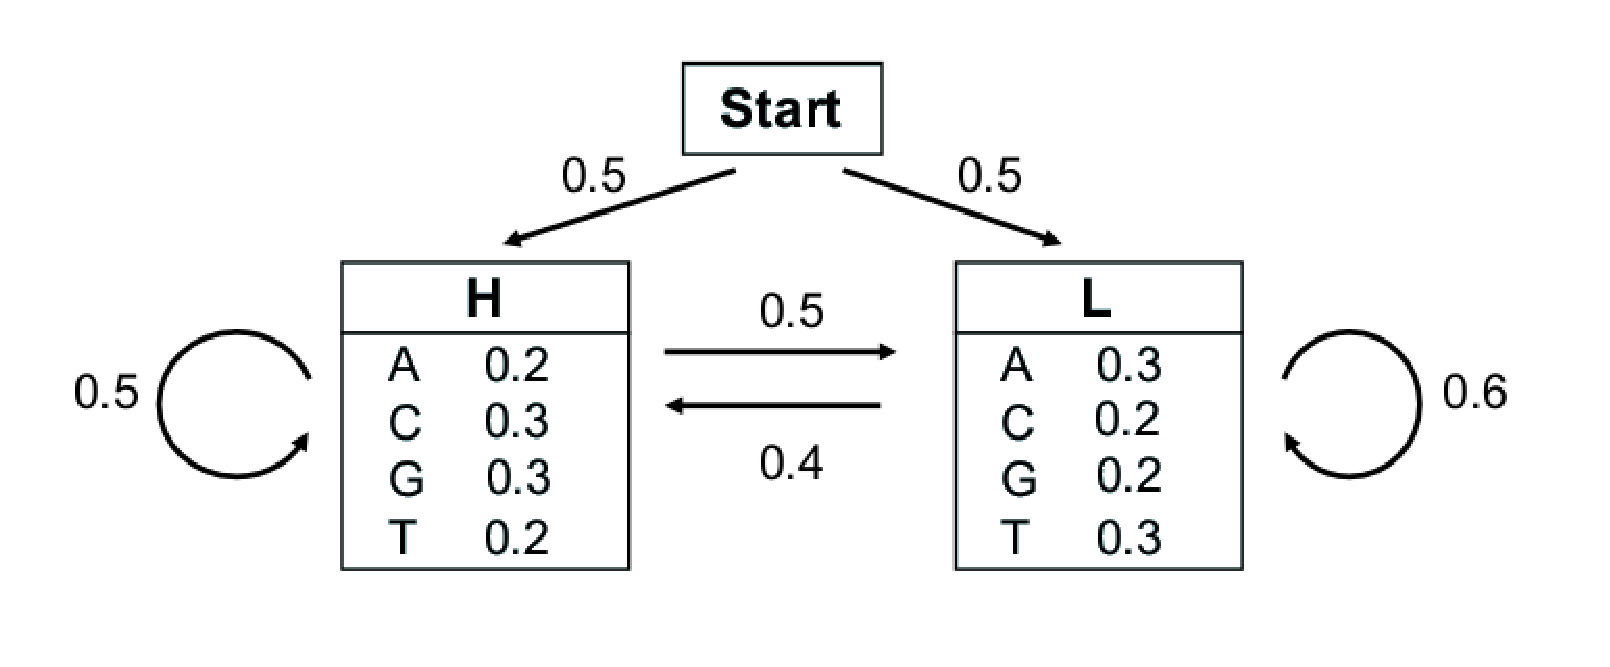
\includegraphics[scale=0.45]{HMM.eps}}
\centerline{\caption{fig}{Figure 1: Hidden Markov Model Example}}\\

The Viterbi calculations are done using sums of $log_2$ probabilities.
\subsection{Viterbi Algorithm}
To calculate the probability of the occurrence of the desired sequence, state transition probability and individual state occurrence probability is calculated. The probabilities of various paths is calculated as there are more than one path to the desired sequence of states. The Viterbi algorithm is a dynamical programming algorithm that computes the most probable path. \\

Consider a HMM with k states. The probability of the most probable path ending in state $l$ with observation $i$ is: 
\begin{equation}
	p_l(i,x) = e_l(i) \cdot \displaystyle\max_k(p_k(j,x-1) \cdot p_{kl})
\end{equation}
where $e_l(i)$ is the  probability to observe element i in state l. $p_k(j,x-1)$ is the probability of the most probable path ending at position x-1 in state k with element j. $p_{kl}$ is probability of the transition from state l to state k. \\

For the given sequence \lq\lq{GGCACTGAA}\rq\rq{}, the probability of the most probable path ending in state \lq{H}\rq{} with observation \lq{A}\rq{} at the fourth position (given C at third position) is calculated as:

\begin{equation}
	p_H(A,4) = e_H(A) \cdot max(p_L(C,3) \cdot p_{LH}, p_H(C,3) \cdot p_{HH} )
\end{equation}
\subsection{Backtracking}
Once the probabilities for all possible states are calculated, the path to the maximum probability is backtracked to find the best path. The state with the highest probability is chosen. In cases where both the states have the same probability value, same path as the previous state is maintained. 
\section{Results}
In this section the results of the two sequences are mentioned in the tables and the most probable path for both the sequence is calculated by taking the max probabilities. $log_2$ probabilities are considered for calculation.
\subsection{Input Sequence 1} 
\begin{center}
\begin{tabular}{ | m{5em} | m{3em} | m{3em} | m{3em} | m{3em} | m{3em} | m{3em} | m{3em} | m{3em} | m{3em} | }
 \hline
 Input Sequence & G & G & C & A & C & T & G & A & A \\
 \hline
 State H & \textbf{-2.73} & \textbf{-5.47} & \textbf{-8.21} & -11.53 & -14.00 & -17.32 & -19.53 & -22.86 & -25.65  \\
 \hline
 State L & -3.32 & -6.05 & -8.79 & \textbf{-10.94} & \textbf{-14.00} & \textbf{-16.48} & \textbf{-19.53} & \textbf{-22.01} & \textbf{-24.48} \\
 \hline
 Best Path & H & H & H & L & L & L & L & L & L \\
 \hline
\end{tabular}
\captionof{table}{Table of maximum probabilities for sequence \lq\lq{GGCACTGAA}\rq\rq{} }
\label{Table:1}
\end{center}
The best probable path for the sequence \lq\lq{GGCACTGAA}\rq\rq{} is HHHLLLLLL and the maximum probability for that sequence is $2^{-24.48}$ = $4.2517\times10^{-08}$. The boldfaced numbers represent the highest probability for the sequence is shown in Table \ref{Table:1}.

\subsection{Input Sequence 2} 

\begin{center}
\begin{tabular}{ | m{5em} | m{3em} | m{3em} | m{3em} | m{3em} | m{3em} | m{3em} | m{3em} | m{3em} | m{3em} | }
 \hline
 Input Sequence & T & C & A & G & C & G & G & C & T \\
 \hline
 State H & -3.32 & -5.79 & -9.11 & \textbf{-11.32} & \textbf{-14.06} & \textbf{-16.80} & \textbf{-19.53} & \textbf{-22.27} & -25.59  \\
 \hline
 State L & \textbf{-2.73} & \textbf{-5.79} & \textbf{-8.26} & -11.32 & -14.38 & -17.38 & -20.12 & -22.86 & \textbf{-25.01} \\
 \hline
 Best Path & L & L & L & H & H & H & H & H & L \\
 \hline
\end{tabular}
\captionof{table}{Table of maximum probabilities for sequence \lq\lq{TCAGCGGCT}\rq\rq{} }
\label{Table:2}
\end{center}
The best probable path for the sequence \lq\lq{TCAGCGGCT}\rq\rq{} is LLLHHHHHL and the maximum probability for that sequence is $2^{-25.01}$ = $2.9525\times10^{-08}$. The boldfaced numbers represent the highest probability for the sequence is shown in Table \ref{Table:2}. 
\section{Conclusion}
The Viterbi algorithm is used to compute the most probable path. It requires knowledge of the parameters of the HMM model and a particular output sequence and it finds the state sequence that is most likely to have generated that output sequence. It works by finding a maximum over all possible state sequences. \\

The same output sequence can be obtained by going through many state sequences but their probabilities will be different. It is possible to calculate the probability for the HMM model to generate that output sequence by doing the summation over all possible state sequences. \\

Using the Viterbi algorithm, the best path for the sequence \lq\lq{GGCACTGAA}\rq\rq{} is HHHLLLLLL and for the sequence \lq\lq{TCAGCGGCT}\rq\rq{} the best path is LLLHHHHHL.
\section{Appendix}
\begin{verbatim}
%Submitted by Rahil Modi - C14109603
clc
clear all
close all
%Order = A,C,G,T
H = log2( [0.2, 0.3, 0.3, 0.2] );
L = log2( [0.3, 0.2, 0.2, 0.3] );

%Initial probability
pl_0 = log2(0.5);
ph_0 = log2(0.5);

%Transition probabilities
phh = log2(0.5);
phl = log2(0.5);
pll = log2(0.6);
plh = log2(0.4);
    
%Input sequence  
%S = ['G', 'G', 'C', 'A', 'C', 'T', 'G', 'A', 'A' ]; %Sequence 1
S = ['T', 'C', 'A', 'G', 'C', 'G', 'G', 'C', 'T' ]; %Sequence 2
size = length(S);
S_a  = zeros(1,size);

%Probabilities 
p              = zeros(4, size);
most_prob_path = zeros(1, size);

%Convert sequence to array
for i = 1:length(S)
   if(S(i) == 'A')
       S_a(i) = 1;
   elseif(S(i) == 'C')
       S_a(i) = 2;
   elseif(S(i) == 'G')
       S_a(i) = 3;
   else
       S_a(i) = 4;
   end
end
%Calculating the forward Probabilities using Viterbi Algorithm
size = length(S_a);  
for i = 1:size
    if( i == 1)
        p(1,i) = ph_0 + H(S_a(i));
        p(2,i) = pl_0 + L(S_a(i));
        if( p(1,i) == p(2,i) )
            p(3,i) = p(1,i);        %Equal
            p(4,i) = 2;             
        elseif(p(1,i) > p(2,i))
            p(3,i) = p(1,i);        %High
            p(4,i) = 0;
        else
            p(3,i) = p(2,i);        %Low
            p(4,i) = 1; 
        end
    else
        p(1,i) = H(S_a(i)) + max ( (p(1, i-1) + phh), (p(2, i-1) + plh) );
        p(2,i) = L(S_a(i)) + max ( (p(1, i-1) + phl), (p(2, i-1) + pll) );
        if( p(1,i) == p(2,i) )
            p(3,i) = p(1,i);        %Equal
            p(4,i) = 2;             
        elseif(p(1,i) > p(2,i))
            p(3,i) = p(1,i);        %High
            p(4,i) = 0;
        else
            p(3,i) = p(2,i);        %Low
            p(4,i) = 1; 
        end
    end
end
%Backtracking
init       = 1;
final_prob = p(4,:);
size       = length(final_prob);
for i = size:-1:1
    if(final_prob(i) == 2)
        if(i == size)
            most_prob_path(i) = init; %If last prob is same, initialize
        else
            most_prob_path(i) = most_prob_path(i+1);
        end
    elseif(final_prob(i) == 0)
        most_prob_path(i) = 0;        %Low
    else
        most_prob_path(i) = 1;        %High
    end
end
disp("Best Probabilities: ");
disp(p(3,:))

for i = 1:size
    if(most_prob_path(i) == 1)
        Ans(i) = 'L';
    else
        Ans(i) = 'H';
    end
end
disp("The most probable path is:")
disp(Ans);
\end{verbatim}
\end{document}